\documentclass[tikz,border=8pt]{standalone}
\usetikzlibrary{arrows.meta,calc}
\definecolor{bg}{HTML}{F7F8FA}
\definecolor{grid}{HTML}{E3E6EB}
\definecolor{link}{HTML}{E9EDF2}
\definecolor{linkedge}{HTML}{5B6773}
\definecolor{linkshade}{HTML}{BFC8D2}
\definecolor{joint}{HTML}{F4A261}
\definecolor{jointedge}{HTML}{B8632A}
\definecolor{pitch}{HTML}{2A6F97}
\definecolor{roll}{HTML}{C0392B}
\definecolor{yaw}{HTML}{2E8B57}
\definecolor{label}{HTML}{233044}
\definecolor{base}{HTML}{6B7A88}
\begin{document}
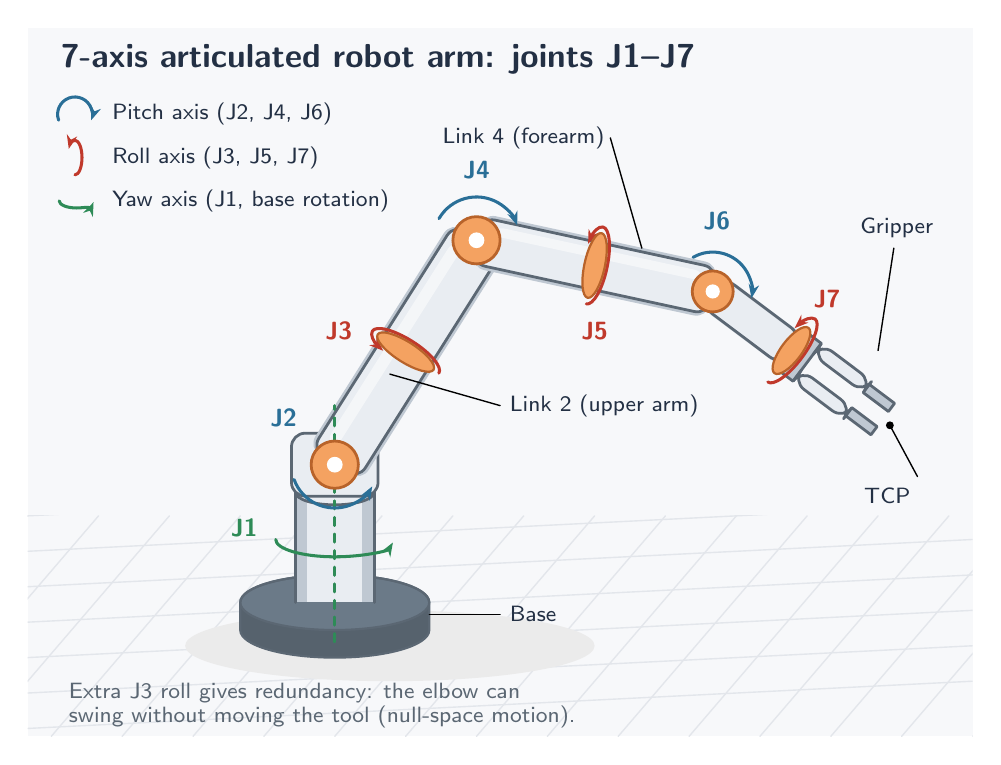
\begin{tikzpicture}[x=1cm,y=1cm,line join=round,line cap=round,
  linkstyle/.style={draw=linkedge,fill=link,line width=1pt,rounded corners=5pt},
  jointstyle/.style={draw=jointedge,fill=joint,line width=1pt},
  axisarrow/.style={-{Stealth[length=5pt]},line width=1.1pt},
  jl/.style={font=\sffamily\bfseries\small,text=label},
  note/.style={font=\sffamily\footnotesize,text=label}]
  \fill[bg] (-0.4,-0.6) rectangle (11.6,8.4);
  \node[font=\sffamily\bfseries\large,text=label,anchor=west] at (-0.1,8.0) {7-axis articulated robot arm: joints J1--J7};

  % ---- floor grid for depth ----
  \begin{scope}
    \clip (-0.4,-0.6) rectangle (11.6,2.2);
    \foreach \i in {-6,...,14}{\draw[grid,line width=0.5pt] (\i*0.9-1,-0.6) -- (\i*0.9+1.4,2.2);}
    \foreach \j in {0,...,6}{\draw[grid,line width=0.5pt] (-0.4,\j*0.45-0.5) -- (11.6,\j*0.45+0.1);}
  \end{scope}

  % ---- shadow ----
  \fill[black!8] (4.2,0.55) ellipse (2.6 and 0.45);

  % ---- base (cylinder with perspective) ----
  \fill[base!80!black] (2.3,0.75) rectangle (4.7,1.1);
  \fill[base] (3.5,1.1) ellipse (1.2 and 0.35);
  \fill[base!80!black] (3.5,0.75) ellipse (1.2 and 0.35);
  \fill[base!80!black] (2.3,0.75) rectangle (4.7,1.1);
  \fill[base] (3.5,1.1) ellipse (1.2 and 0.35);
  \draw[linkedge,line width=0.8pt] (2.3,0.75) arc (180:360:1.2 and 0.35) -- (4.7,1.1) arc (0:180:1.2 and 0.35) -- cycle;
  \draw[linkedge,line width=0.8pt] (3.5,1.1) ellipse (1.2 and 0.35);
  % column (J1 rotates about vertical axis)
  \fill[linkshade] (3.0,1.1) rectangle (4.0,2.5);
  \fill[link] (3.15,1.1) rectangle (3.85,2.5);
  \draw[linkedge,line width=1pt] (3.0,1.1) -- (3.0,2.5) (4.0,1.1) -- (4.0,2.5);
  \fill[link,draw=linkedge,line width=1pt] (3.5,2.5) ellipse (0.5 and 0.16);

  % ---- link geometry (2D pose with 3D shading) ----
  % shoulder block
  \filldraw[linkstyle] (2.95,2.45) rectangle (4.05,3.25);
  % upper arm: J2 (3.5,2.85) -> J4 (5.3,5.7)
  \begin{scope}[rotate around={57.7:(3.5,2.85)}]
    \fill[linkshade,rounded corners=5pt] (3.5,2.45) rectangle (6.9,3.25);
    \filldraw[linkstyle] (3.5,2.5) rectangle (6.9,3.2);
    \fill[white,opacity=0.5,rounded corners=3pt] (3.7,2.95) rectangle (6.7,3.1);
  \end{scope}
  % forearm: J4 (5.3,5.7) -> J6 (8.3,5.05)
  \begin{scope}[rotate around={-12.2:(5.3,5.7)}]
    \fill[linkshade,rounded corners=5pt] (5.3,5.35) rectangle (8.37,6.05);
    \filldraw[linkstyle] (5.3,5.4) rectangle (8.37,6.0);
    \fill[white,opacity=0.5,rounded corners=3pt] (5.5,5.8) rectangle (8.2,5.92);
  \end{scope}
  % wrist: J6 (8.3,5.05) -> J7 (9.3,4.3)
  \begin{scope}[rotate around={-36.9:(8.3,5.05)}]
    \fill[linkshade,rounded corners=4pt] (8.3,4.8) rectangle (9.55,5.3);
    \filldraw[linkstyle] (8.3,4.82) rectangle (9.55,5.28);
  \end{scope}
  % flange + gripper beyond J7
  \begin{scope}[rotate around={-36.9:(9.3,4.3)}]
    \filldraw[draw=linkedge,fill=linkshade,line width=1pt] (9.3,4.0) rectangle (9.55,4.6);
    \filldraw[linkstyle] (9.55,4.42) rectangle (10.35,4.6);
    \filldraw[linkstyle] (9.55,4.0) rectangle (10.35,4.18);
    \filldraw[draw=linkedge,fill=linkshade,line width=1pt] (10.35,4.42) rectangle (10.75,4.55);
    \filldraw[draw=linkedge,fill=linkshade,line width=1pt] (10.35,4.05) rectangle (10.75,4.18);
  \end{scope}

  % ---- joints ----
  % J1 (yaw, vertical axis) drawn as ring on the column
  \draw[yaw,line width=1pt,dashed] (3.5,0.6) -- (3.5,3.6);
  \draw[axisarrow,yaw] (2.75,1.9) arc (180:350:0.75 and 0.22);
  \node[jl,text=yaw] at (2.35,2.05) {J1};

  % J2 pitch at shoulder
  \filldraw[jointstyle] (3.5,2.85) circle (0.3);
  \fill[white] (3.5,2.85) circle (0.1);
  \draw[axisarrow,pitch] (3.5,2.85) ++(200:0.55) arc (200:330:0.55);
  \node[jl,text=pitch] at (2.85,3.45) {J2};

  % J3 roll around the upper arm
  \begin{scope}[rotate around={57.7:(4.4,4.28)}]
    \draw[axisarrow,roll] (4.4,4.28) ++(0.0,-0.5) arc (-90:150:0.16 and 0.5);
  \end{scope}
  \filldraw[draw=jointedge,fill=joint,line width=0.8pt,rotate around={57.7:(4.4,4.28)}] (4.4,4.28) ellipse (0.13 and 0.42);
  \node[jl,text=roll] at (3.55,4.55) {J3};

  % J4 pitch at elbow
  \filldraw[jointstyle] (5.3,5.7) circle (0.3);
  \fill[white] (5.3,5.7) circle (0.1);
  \draw[axisarrow,pitch] (5.3,5.7) ++(150:0.55) arc (150:20:0.55);
  \node[jl,text=pitch] at (5.3,6.6) {J4};

  % J5 roll around the forearm
  \begin{scope}[rotate around={-12.2:(6.8,5.38)}]
    \draw[axisarrow,roll] (6.8,5.38) ++(0.0,-0.5) arc (-90:150:0.16 and 0.5);
  \end{scope}
  \filldraw[draw=jointedge,fill=joint,line width=0.8pt,rotate around={-12.2:(6.8,5.38)}] (6.8,5.38) ellipse (0.13 and 0.42);
  \node[jl,text=roll] at (6.8,4.55) {J5};

  % J6 pitch at wrist
  \filldraw[jointstyle] (8.3,5.05) circle (0.26);
  \fill[white] (8.3,5.05) circle (0.09);
  \draw[axisarrow,pitch] (8.3,5.05) ++(120:0.5) arc (120:-10:0.5);
  \node[jl,text=pitch] at (8.35,5.95) {J6};

  % J7 roll of the flange
  \begin{scope}[rotate around={-36.9:(9.3,4.3)}]
    \draw[axisarrow,roll] (9.3,4.3) ++(0.0,-0.5) arc (-90:150:0.16 and 0.5);
  \end{scope}
  \filldraw[draw=jointedge,fill=joint,line width=0.8pt,rotate around={-36.9:(9.3,4.3)}] (9.3,4.3) ellipse (0.13 and 0.36);
  \node[jl,text=roll] at (9.75,4.95) {J7};

  % ---- tool centre point ----
  \fill[label] (10.55,3.35) circle (0.05);
  \draw[label,line width=0.5pt] (10.55,3.35) -- (10.9,2.7);
  \node[note,anchor=west] at (10.1,2.45) {TCP};

  % ---- part labels (base / links / end effector) ----
  \draw[label,line width=0.5pt] (4.7,0.95) -- (5.6,0.95);
  \node[note,anchor=west] at (5.6,0.95) {Base};
  \draw[label,line width=0.5pt] (4.2,4.0) -- (5.6,3.6);
  \node[note,anchor=west] at (5.6,3.6) {Link 2 (upper arm)};
  \draw[label,line width=0.5pt] (7.4,5.6) -- (7.0,7.0);
  \node[note,anchor=east] at (7.05,7.0) {Link 4 (forearm)};
  \draw[label,line width=0.5pt] (10.4,4.3) -- (10.6,5.6);
  \node[note,anchor=west] at (10.05,5.85) {Gripper};

  % ---- legend ----
  \draw[axisarrow,pitch] (0.2,7.3) ++(200:0.22) arc (200:-20:0.22);
  \node[note,anchor=west] at (0.55,7.3) {Pitch axis (J2, J4, J6)};
  \draw[axisarrow,roll] (0.2,6.75) ++(-90:0.22) arc (-90:150:0.09 and 0.22);
  \node[note,anchor=west] at (0.55,6.75) {Roll axis (J3, J5, J7)};
  \draw[axisarrow,yaw] (0.0,6.2) arc (180:350:0.22 and 0.09);
  \node[note,anchor=west] at (0.55,6.2) {Yaw axis (J1, base rotation)};
  \node[note,anchor=west,text=linkedge] at (0.0,-0.05) {Extra J3 roll gives redundancy: the elbow can};
  \node[note,anchor=west,text=linkedge] at (0.0,-0.35) {swing without moving the tool (null-space motion).};
\end{tikzpicture}
\end{document}
